\documentclass[a4paper]{article}
\usepackage[a4paper,margin=0.3in,landscape]{geometry}

\setlength{\columnseprule}{0.3pt}

% default stuff
\usepackage{amsmath}
\usepackage{amssymb}
\usepackage{enumitem}

% multicolumn package
\usepackage{multicol}

\usepackage{multirow}
\usepackage{makecell}
\renewcommand\theadfont{\bfseries}

\newcolumntype{M}[1]{>{\centering\arraybackslash} m{#1}} % centered m

\newcommand{\abs}[1]{\left\lvert#1\right\rvert}

\newcommand{\ol}[1]{\begin{enumerate}#1\end{enumerate}}
\newcommand{\oll}[1]{\begin{enumerate}[leftmargin=*]#1\end{enumerate}}
\newcommand{\ul}[1]{\begin{itemize}#1\end{itemize}}
\newcommand{\ull}[1]{\begin{itemize}[leftmargin=*]#1\end{itemize}} % no margin


% red
\usepackage[dvipsnames,table]{xcolor}
\newcommand{\red}[1]{\textcolor{red}{#1}}

% unit
\newcommand{\unit}[1]{\ensuremath{\, \mathrm{#1}}}

% inverse
\newcommand{\inv}{^{-1}}

\usepackage{graphicx}
\graphicspath{ {./images/} }

\pagenumbering{gobble}

\AtBeginDocument{
\addtolength{\abovedisplayskip}{-1ex}
\addtolength{\abovedisplayshortskip}{-1ex}
\addtolength{\belowdisplayskip}{-1ex}
\addtolength{\belowdisplayshortskip}{-1ex}
}

% reduce spacing before and after headers
\makeatletter
\renewcommand{\section}{
  \@startsection{section}{1}{0pt}{1ex}{1.2ex}{\normalfont\large\bfseries}}
\renewcommand{\subsection}{
  \@startsection{subsection}{2}{0pt}{1ex}{1.2ex}{\normalfont\normalsize\bfseries}}
% 5th arg is different for paragraph
\renewcommand{\paragraph}{
  \@startsection{paragraph}{4}{0pt}{1.5ex}{-0.8em}{\normalfont\bfseries}}

% TODO
% Page limit: 4
% - add units for Lec 10 to 12

\begin{document}
\begin{multicols*}{4}
  \small
  \part*{\centering \underline{PC1201 E\&M}}
  \section*{\underline{Misc}}
    \subsection*{Charges}
      \paragraph{Net charge} An object is
        \ull {
          \item +vely charged if it has an excess of protons
          \item -vely charged if it has an excess of electrons
          \item Neutral otherwise
          \item \red{has units \unit{C}}
        }
      \paragraph{Conservation of charge} One cannot create/destroy charges; one can only transfer charges from one body to another
      \paragraph{Interaction} Like charges repel, unlike charges attract
      \paragraph{L12 QC6} 
        \ull {
          \item Charges move because of a PD
          \item If two conductors are connected via a wire, charges redistribute equally only if the two conductors are identical.
        }
    \subsection*{Insulators}
      \paragraph{Definition} Do not allow electrons to flow freely
      \paragraph{Charging} By friction molecular bonds are broken, allowing a neutral molecule to split into positive and negative parts
    \subsection*{Conductors}
      \paragraph{Definition} Allow electrons to flow freely
      \paragraph{Polarization} Charged object brought near to a conductor. Freely moving electrons will congregate accordingly to one side of the conductor
      \paragraph{Charging by contact} Touch a conductor with an initially charged object. Charges will spread through the conductor. The initially charged object gets discharged
      \paragraph{Grounding} Electrons will flow to the object that is ``more positive''
      \paragraph{Charging by induction} Polarization with grounding on the opposite side
  \section*{\underline{Electric force}}
    \ull {
      \item $\vec{F}_{ab}$ is the force on $a$ due to $b$
      \item Is a vector, so can apply superposition
    }
    \subsection*{Coulomb's law}
      \paragraph{Magnitude} For two charges $q_1$ and $q_2$ seperated by distance $r$:
      \[ \abs{\vec{F}_{12}} = \abs{\vec{F}_{21}} = \frac{k \abs{q_1} \abs{q_2}}{r^2} \]
      \paragraph{Direction}
        \ull {
          \item Along the line joining two charges
          \item Unlike charges attract; like charges repel
        }
      \paragraph{Superposition} Electric force on a charge is the \red{vector} sum of the individual force due to all the other charges
      \paragraph{Limitations}
        \ull {
          \item Only applies to point charges, but objects may be modeled as point charges if the $r$ is much larger than their size
          \item Only applies to static charges, but this module focuses on static charges
        }
  \section*{\underline{E-field}} \noindent
    \ull {
      \item Explains how a charge can be aware of the presence of another charge
      \item Force is exerted on a charged object, while field is exerted on a point in space
      \item \red{has units \unit{NC\inv} or \unit{Vm\inv}}
    }
    \subsection*{E-field for a point charge}
      \paragraph{Magnitude} We obtain magnitude by placing a test charge at the point we are interested in.
        \[ \abs{\vec{E}} = \frac{\abs{\vec{F}}}{q_\text{test}} = \frac{k \abs{q_0}}{r^2} \]
        where $q_0$ is the charge that created the e-field.
      \paragraph{Direction} Defined to be the direction of the force experienced by a positive $q_\text{test}$
        \begin{center}
          \begin{tabular}{ |c|c|c| }
            \hline
            & +ve $q_\text{test}$ & -ve $q_\text{test}$ \\ \hline
            Field & Points away & Points towards \\ \hline
            Force & \makecell{Same dir.\\as field} & \makecell{Opposite dir.\\from field} \\ \hline
          \end{tabular}
        \end{center}
        \paragraph{Superposition} E-field at a point is the \red{vector} sum of the individual fields due to all the charges
    \subsection*{E-field lines} \noindent
      Exist at every point in space, just a representative sample
      \paragraph{Magnitude} Higher density of field lines $\Rightarrow$ stronger field
      \paragraph{Direction}
        \ull {
          \item E-field vector is tangent to e-field line
          \item Field lines do not cross
          \item Field lines start from +ve charges and end at -ve charges
        }
    \subsection*{E-field for sphere} \noindent
      Let $R$ be the radius of the sphere. The following applies to:
      \ull {
        \item Thin insulating shell with uniform distribution
        \item Thin conducting shell (assume no charge nearby)
        \item Conducting sphere (assume no charge nearby)
      }
      \paragraph{Outside sphere} Let $Q$ be the total charge on the sphere. Let $r$ be the distance to the centre of the sphere.
        \[ \abs{\vec{E}} = \frac{k\abs{Q}}{r^2} \]
      \paragraph{Inside sphere} Inside the sphere, there is no e-field due to symmetry
    \subsection*{E-field for infinite sheet/plate}
      \ull {
        \item We can approximate most large sheets/plates as infinite sheets/plates
        \item We use this setup for parallel plate capacitors
      }
      \paragraph{Magnitude} Let $Q$ be the total charge on the plate. Let $A$ be the area of each plate
        \[ \abs{\vec{E}} = \frac{\abs{Q}}{2 \varepsilon_0 A} \]
    \subsection*{E-field for dipole}
      \paragraph{Direction} \noindent \\
        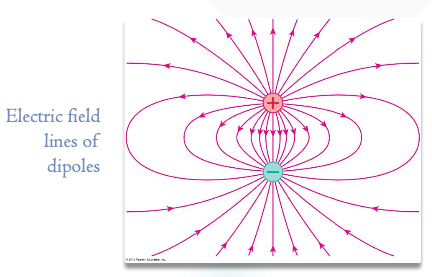
\includegraphics[width=0.24\textwidth]{dipole_field_lines}
    \subsection*{E-field in conductors}
      \ull {
        \item We only consider conductors in electric equilibrium, so $\vec{E} = 0$
        \item Excess charges reside only on the surface, congregating at sharp points
        \item E-fields are perpendicular to surface
      }
    \subsection*{Misc}
      \paragraph{Dielectric breakdown} When e-fields within insulators get too strong, it may fail to act as an insulator, turning into a conductor, allowing charges to flow
      \paragraph{Screening in conductors} When conductors are placed in an e-field, as mentioned previously, $\vec{E} = 0$, so any void in the conductor will also have $\vec{E} = 0$ (Faraday's cage / electrostatic shielding)
  \section*{\underline{Electric potential energy}}
    \subsection*{Interaction EPE for a point charge}
      \paragraph{Magnitude} A charge $q_1$ will have PE if another charge $q_2$ is present
        \[ U_{q_1} = \frac{k q_1 q_2}{r} = U_{q_2} \]
      \paragraph{Alternative} Based on the definition of electric potential later, we also have
        \[ \Delta U = q \Delta V \]
      \paragraph{Zero point} $U \rightarrow 0$ as $r \rightarrow \infty$, i.e. when there are no charges around
      \paragraph{Sign}
        \ull {
          \item Similar charges have positive $U$, while opposite charges have negative $U$.
          \item Not a vector, so has no direction
        }
      \paragraph{Superposition} EPE due to multiple charges is the \red{scalar} sum of individual terms
    \subsection*{Interaction EPE vs electric force} \noindent
      \paragraph{$\Delta U$ vs $\vec{F}_\text{ext}$}
        Work done is given by
        \[ W = \vec{F}_\text{ext} d \cos\theta \]
        where $d$ is usually positive in the direction of displacement, and $\theta$ is the angle between $\vec{F}_\text{ext}$ and $d$. We can also define work done as
        \[ W = \Delta U = U_f - U_i \]
        Hence,
        \ull {
          \item $\theta = 0 \Rightarrow$ same dir. $\Rightarrow W = \vec{F}_\text{ext} d > 0 \Rightarrow \Delta U > 0$
          \item $\theta = 180 \Rightarrow$ diff dir. $\Rightarrow W = \vec{F}_\text{ext} d < 0 \Rightarrow \Delta U < 0$
        }
        Here, $\Delta U$ is the work done on the charge to bring it from initial point $i$ to final point $f$.
      \paragraph{$\Delta U$ vs Coulomb's force $\vec{F}$}
        In order to move the charged object at constant velocity, we have to oppose Coulomb's force, so
        \[ \vec{F} = -\vec{F}_\text{ext} \]
        This case has a negative sign, so
        \ull {
          \item $\vec{F}$ and $d$ same dir. $\Rightarrow \Delta U < 0$
          \item $\vec{F}$ and $d$ diff dir. $\Rightarrow \Delta U > 0$
        }
    \subsection*{Configuration EPE} \noindent
      Work required to bring the charges from infinity to build this configuration
      \[ U = \sum_{i<j} \frac{k q_i q_j}{r_{ij}} \]
  \section*{\underline{Electric potential}}
    \ull {
      \item Like e-field, electric potential explains how a charge can be aware of the presence of another charge
      \item But e-field is about \red{force per charge} while electric potential is about \red{work done/energy per charge}
      \item \red{has units \unit{V}}
    }
    \subsection*{Electric potential for a point charge}
      \paragraph{Magnitude} Similar to e-field, we obtain magnitude by placing a test charge at the point we are interested in.
        \[ V = \frac{U}{q_\text{test}} = \frac{k q_0}{r} \]
        where $q_0$ is the charge that created the electric potential.
      \paragraph{Zero point} We can choose the zero point of $V$.
      \paragraph{Superposition} Electric potential at a point is the \red{scalar} sum of potential due to each charge
    \subsection*{Electric potential for a sphere/shell} \noindent
      Let $R$ be the radius of the sphere. The following applies to:
      \ull {
        \item Thin insulating shell with uniform distribution
        \item Thin conducting shell (assume no charge nearby)
        \item Conducting sphere (assume no charge nearby)
      }
      \paragraph{Outside sphere} Let $Q$ be the total charge on the sphere. Let $r$ be the distance to the centre of the sphere.
        \[ V = \frac{kQ}{r} \]
      \paragraph{Inside sphere} Inside the sphere, potential is constant.
        \[ V = \frac{kQ}{R} \]
    \subsection*{Equipotential surfaces}
      \ull {
        \item Lines/surfaces of the same potential, so moving a charge along the line does not change EPE
        \item PD between each adjacent pair of equipotential lines is the same
      }
    \subsection*{Relationship to $\vec{E}$}
      \ull {
        \item E-field points in direction of decreasing potential, so a PD causes an $\vec{E}$
        \item E-fields are perpendicular to equipotential lines
        \item If E-field is constant, then
          \[ \abs{\vec{E}} = \frac{\abs{\Delta V}}{d} \]
          where $d$ is the distance between the two points (parallel to $\vec{E}$), and $\Delta V$ is the PD between the two points.
        \begin{center}
          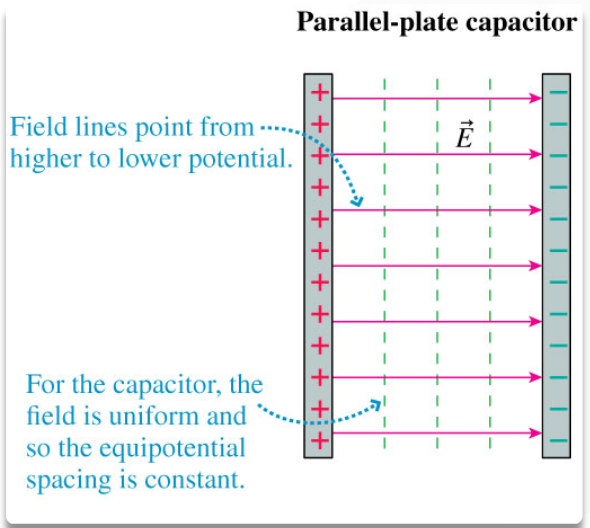
\includegraphics[width=0.2\textwidth]{potential_and_e_field}
        \end{center}
      }
    \subsection*{Moving charge in a field}
      \oll {
        \item Charge $q$ moving from A to B in a PD $\Delta V$
          \[ \Delta U = q \Delta V \]
        \item Charge $q$ moving from A to B in a \red{constant} $\vec{E}$ field
          \[ \vec{\Delta V} = \abs{\vec{E}} d \]
      }
  \section*{\underline{Capacitance, current, resistance}}
    \subsection*{Capacitor}
      \paragraph{Capacitance} A capacitor stores electric charges, and consists of two equally and oppositely charged parts, that are some distance apart. The capacitance $C$ is given as:
        \[ C = \frac{Q}{\Delta V} = \kappa \frac{\varepsilon_0 A}{d} \]
        \ull {
          \item $Q$ is the amount of charge the capacitor can hold, given PD between the plates $\Delta V$
          \item $\kappa$ is the dielectric constant, 1 in air, others will be given
          \item RHS is always true, even if the capacitor is disconnected
          \item \red{has units \unit{CV\inv} or \unit{F}}
        }
      \paragraph{Electric field} Proved in assignment 2:
        \[ \abs{\vec{E}} = \frac{Q}{\varepsilon_0 A} \]
      \paragraph{Energy} Energy stored in a capacitor is equal to the work done to charge it
        \[ U = \frac{1}{2} Q \Delta V = \frac{Q^2}{2C} = \frac{1}{2} C (\Delta V)^2 \]
      \paragraph{Energy density} The capacitor's energy is stored in the electric field between the plates.
        \[ U = \frac{1}{2} C (\Delta V)^2 = \frac{1}{2} \frac{\varepsilon_0 A}{d} (Ed)^2 = \frac{1}{2} \varepsilon_0 E^2 (Ad) \]
        In order to be independent of the dimensions of the capacitor, define $u = \dfrac{U}{Ad}$ to be the energy density, so we have
        \[ u = \frac{1}{2} \varepsilon_0 E^2 \]
    \subsection*{Current}
      \ull {
        \item Rate of flow of charge
          \[ I = \frac{Q}{\Delta t} \]
        \item \red{has units \unit{Cs\inv} or \unit{A}}
        \item Direction of flow of positive charges
        \item Charges flow $\Rightarrow \Delta V$ exists $\Rightarrow$ electric field exists
      }
      \paragraph{EMF source, $\varepsilon$}
        \ull {
          \item Maintains a constant PD by moving charges against the electric field, opposing Coulomb's force
          \item \red{has units \unit{V}}
        }
      \paragraph{Power}
        \[ P = \frac{U}{\Delta t} = \frac{q \Delta V}{\Delta t} = I \Delta V = I \varepsilon \]
    \subsection*{Resistance}
      \ull {
        \item For ohmic materials, which have constant resistance, Ohm's law holds true:
          \[ R = \frac{\Delta V}{I} \]
        \item Can assume the materials are ohmic unless otherwise stated
        \item \red{has units \unit{\Omega} or \unit{VA\inv}}
      }
      \paragraph{Computing resistance for a material}
        \[ R = \frac{\rho l}{A} \]
        where $\rho$ is the resistivity (given), $l$ is the length of the conductor, $A$ is the cross sectional area.
      \paragraph{Power} For ohmic resistors,
        \[ P = I^2 R = \frac{(\Delta V)^2}{R} \]
        Power ratings in household appliances are based off a constant voltage (230V in Singapore)
  \section*{\underline{DC Circuits}}
    \paragraph{Battery} Positive terminal is the longer line
      \subsection*{Resistors}
        \begin{center}
          \begin{tabular}{ |c|c|c| }
            \hline
            & Series & Parallel \\ \hline
            PD & Sum & Same \\ \hline
            Current & Same & Sum \\ \hline
            Resistance & Sum & \makecell{Reciprocal of \\ (sum of reciprocals)} \\ \hline
          \end{tabular}
        \end{center}
      \subsection*{Capacitor}
        \begin{center}
          \begin{tabular}{ |c|c|c| }
            \hline
            & Series & Parallel \\ \hline
            PD & Sum & Same \\ \hline
            Charge & Same & Sum \\ \hline
            Capacitance & \makecell{Reciprocal of \\ (sum of \\ reciprocals)} & Sum \\ \hline
          \end{tabular}
        \end{center}
      \subsection*{Kirchhoff}
        \paragraph{Parallel vs series}
          \ull {
            \item Two elements are in \red{parallel} if \red{any} loop contains only those two elements
            \item Two elements are in \red{series} if \red{every} loop contains only both those elements
          }
        \paragraph{Junction rule} charge in = charge out
        \paragraph{Loop rule}
          \ull {
            \item Loop rule: sum of PD along loop is 0
            \item Battery: Positive plate has higher potential than negative plate
            \item Resistor: Potential decreases in the direction of current (depends on the emf or the setup)
          }
  \section*{\underline{Magnetic field}}
    \ull {
      \item Is a vector, so can apply superposition
      \item \red{has units \unit{T}}
    }
    \paragraph{Magnet}
      \ull {
        \item Has ``inherent magnetic moments'' that are aligned.
        \item This is why dropping/heating will harm the magnet
      }
    \paragraph{Earth is a magnet}
      \ull {
        \item The magnetic north pole is the geographic south pole of the earth
        \item A compass needle points north because the north pole of the compass needle is attracted to the south pole of the earth
      }
    \paragraph{Magnetic field lines}
      \ull {
        \item Starts from north pole, ends at south pole
        \item Denser where field is stronger (near magnet)
        \item Never crosses
      }
    \paragraph{3D convention}
      \ull {
        \item Cross means current into page, dot means current out of page
        \item Vertical plane (up/down, west/east): used in question paper
        \item Horizontal plane (north/south, west/east): surface of the earth
        \item Other plane (up/down, north/south): visualize earth's B-field aways away from the equator
      }
    \subsection*{Source of magnetic fields}
      \paragraph{Right hand grip rule (RHGR)}
        \oll {
          \item Point your right thumb in the direction of current
          \item Wrap your fingers around the wire to indicate a circle
          \item Your fingers curl in the direction of the B-field lines around the wire
        }
      % TODO maybe compress this?
      \paragraph{Moving charge (in a wire)}
        \ull {
          \item Magnitude is
            \[ \abs{\vec{B}} = \frac{\mu_0 I}{2 \pi r} \]
          \item Direction determined by RHGR
        }
      \paragraph{Current loop}
        \ull {
          \item Magnitude at the centre is:
            \[ \abs{\vec{B}} = \frac{\mu_0 N I}{2R} \]
          \item Direction determined by RHGR, or
          \item Fingers curl in the current direction, thumb points in direction of B (magnetic north)
        }
      \paragraph{Solenoid}
        \ull {
          \item Magnitude inside solenoid is almost uniform
            \[ \abs{\vec{B}} = \frac{\mu_0 N I}{L} = \mu_0 n I \]
            where $N$ is the number of turns, and $n = N/L$ is the number of turns per unit length
          \item From Tut 6, $N = L / (2r)$. This $r$ is the radius of the cross-section of the wire, NOT the radius of the solenoid.
          \item Magnitude outside solenoid is very small
          \item Direction: use RHGR like in current loop
        }
  \section*{\underline{Magnetic force}}
    \paragraph{Right hand cross rule (RHCR)}
      \oll {
        \item Point 4 fingers in the direction of $v$
        \item Rotate hand so that palm faces direction of $B$
        \item Direction of thumb is direction of the force $F$
        \item If charge is negative, flip the direction of the force
      }
    \subsection*{Force on moving charge}
      \paragraph{Magnitude}
        \[ \abs{\vec{F}} = \abs{q} v_\perp B = \abs{q} v B \sin \alpha \]
      \paragraph{Direction} use RHCR
      \paragraph{Trajectory}
      \ull {
        \item If initial $v$ is perpendicular to $B$, since $F$ is always perpendicular to $v$, we have circular motion
          \[ F = qvB = \frac{mv^2}{r} \]
        \item Otherwise, there is circular motion in the horizontal plane, but also vertical motion in the vertical axis. This is called helical motion.
      }
    \subsection*{Force on current-carrying wire}
      \paragraph{Magnitude} A wire has $Nq$ charge flowing in it, so we have
        \[ F = Nq vB \sin \alpha \] 
        If we multiply by $t/t$, we have
        \[ F = \frac{Nq}{t} (vt) B \sin \alpha \]
        where $vt$ is the length of the wire, and $I = \dfrac{Nq}{t}$ is the current.
      \paragraph{Direction} use RHCR, replacing $v$ with $I$ (they are in the same direction actually)
    \subsection*{Force between (parallel) current-carrying wires}
      \paragraph{Magnitude} Each wire exerts a force on the other, and it is symmetric:
        \[ F = F_{12} = F_{21} = I_2 l B = I_2 l \left(\frac{\mu_0 I_1}{2 \pi r}\right) \]
        where $r$ is the distance between the wires. Alternatively,
        \[ F = \frac{\mu_0 I_1 I_2 l}{2 \pi r} \]
      \paragraph{Direction} If their currents are flowing in the same direction, then the wires will attract. Otherwise they repel.
    \subsection*{Cross fields} \noindent
      If we want to filter charges, we can pass them through a cross field that has both electric and magnetic forces.
      \paragraph{Direction}
        \ull {
          \item Arrange in such a way that the forces are equal and opposite (for a particular type of charge, e.g. positive), then for the negative charge it will be equal but in the same direction
          \item Thus positive charges will move straight
        }
      \paragraph{Magnitude} We must have $qvB = qE$, i.e.
        \[ v = \frac{E}{B} \]
  \section*{\underline{Induction}}
    \subsection*{Motional EMF}
      \paragraph{How it works}
        \ull {
          \item When a conductor moves perpendicular to a B-field (via $F_\text{ext}$), then $F_B$ is exerted on the charges. But $F_B$ acts in opposite directions for positive and negative charges, so there is a charge separation, leading to an EMF.
          \item The building of the EMF creates a PD, resulting in a $F_E$ that will resist $F_B$. So charges continue accumulating until $F_B = F_E$.
            \begin{align*}
              F_B &= F_E \\
              qvB &= qE \\
              vB &= \frac{\Delta V}{d} \\
              \Delta V &= Bdv
            \end{align*}
            and we rename $\varepsilon = \Delta V$ and $l = d$ to get the more well-known
            \[ \varepsilon = Blv \]
        }
      \paragraph{Induced current} If the moving conductor is connected to a circuit, then a current is induced.
        \[ I = \frac{\varepsilon}{R} = \frac{Blv}{R} \]
      \paragraph{Induced force} With the induced current, and since the conductor is moving in a B-field, we have a magnetic force
        \[ F = IlB = \frac{B^2 l^2 v}{R} \]
        and direction can be obtained via RHCR (with current). Note that $v$ is in the direction of $F_\text{ext}$.
    \subsection*{Magnetic flux} \noindent
      \ull {
        \item Amount of B-field that passes through a loop
        \item Magnitude is
          \[ \phi = NBA \cos \theta \]
          where $N$ is the number of loops, $A$ is the area of the loop, and $\theta$ is the angle between the axis of the loop to the B-field
        \item Axis of the loop is the line passing through the centre of the loop, so $A \cos \theta$ is like the effective area of the loop
        \item \red{has units \unit{Tm^2} or \unit{Wb}}
      }
    \subsection*{Faraday's law} \noindent
      An EMF is induced in a conducting loop if the magnetic flux through the loop changes
      \[ \varepsilon = \abs{\frac{\Delta \phi}{\Delta t}} \]
      and any of $B, A, \theta$ may cause a change in flux.
    \subsection*{Lenz's law} \noindent
      Direction of induced current is such that the induced B-field opposes the change in flux.
      \begin{equation*}
        \resizebox{\hsize}{!}{$
          \Delta \phi \rightarrow \varepsilon_\text{induced} \rightarrow I_\text{induced} \rightarrow B_\text{induced} \rightarrow \phi_\text{induced}
        $}
      \end{equation*}
      \paragraph{How to apply}
        \oll {
          \item Determine direction of B-field
          \item Determine if flux is increasing/decreasing
          \item Lenz's law states that induced B-field will oppose this change
          \item RHGR determines the direction of $I$ that induces this B-field
        }
\end{multicols*}
\end{document}
